%%%%%%%%%%%%%%%%%%%%%%%%%%%%%%%%%%%%%%%%%%%%%%%%%%%%%%%%%%%%%%%%%%%%%%%%%%%%%%%%%%%%%%%%%%%%%%%%%%%
\chapter{Background} \label{ch:Concepts}

\section{Introduction}
In this chapter we will discuss some important concepts relevant to this dissertation. This include the components needed to achieve autonomous navigation, the working principles of the sensors used to perceive the environment and a quick overview of the \ac{ROS} platform.
\section{Autonomous Mobile Robot Sensors}
The most typical type of sensors used for perception in the current state of the art are laser range finders, sonar and 
%GIVE OVERVIEW OF THE CURRENT SENSORS LEADING INDOOR NAVIGATION.

\section {Autonomous Navigation}
There are four main problems associated with robotic autonomous navigation. They are Cognitive Mapping, Localization, Path Planning and Motion Control \cite{baranov2014}. To combat this problems various algorithms have been developed over the years. In the sections bellow we will discuss the main ones used in this dissertation.

\subsection{Mapping}

Creating a map in ROS is typically done by using an improved version of  Rao-Blackwellized particle filters such as the ones described in \cite{grisetti2007improved}. This approach has proven to be an effective way to solve the \ac{SLAM} problem and will be used later on in this work to produce a valid map of our indoor environment.
%gmapping, slam, eurico LASER
\subsection{Localization}
With the grid map built we now need to estimate the robot's position in said map. 
An easy solution to this problem is relying on the robot's odometry information inferred by the robot's encoders and inertial sensors such as accelerometers and gyroscopes. This kind of dead reckoning is an easy and low cost solution for the localization problem. However since the sensor data is integrated over time, this leads to the accumulation of errors which make this approach not feasible for long navigation tasks. 
To fix this issue various algorithms were developed being the most popular ones based on particle filters.
The \ac{AMCL} algorithm  is the standard choice in this case. It takes into account a group of particles, each one corresponding to a certain robot state (position and orientation in this case). As the robot moves the least probable states are filtered out and  the particles should over time converge on the actual position of the robot.  
\subsection{Path Planning}
Assuming the robot can localize itself on the map with a reasonable error we can start sending navigation goals to the robot. To reach the goal the robot must be able to find an optimal path that optimizes the travel distance while avoiding obstacles. The outputted plan can vary depending on the algorithm used. In our case we will use the well known dijaktra algorithm.
\subsection{Motion Control}
After the optimal plan is computed the final step is to compute the best velocity command that will be sent to the base.  In order to do this we will use a similar approach to the one used in \cite{gerkey2008planning}. A set of velocities are simulated during a given set of time and the corresponding predicted trajectories are  computed. For each trajectory it is calculated a determined cost given by a cost function. For each cost th
\section {FMCW radars working principle}
In order to retrieve the best data for our application we first need to understand how the radar works. The following sections will try explain how the radar calculates the range, velocity and angle of an object.
\subsection{range Detection}
An FMCW radar transmits a signal called a “chirp”. A chirp is a sinusoid whose frequency  increases linearly with time.
%% put A t and f t plot
A chirp is characterized by a start frequency (fc), bandwidth(B) and duration (Tc). The slope (S) of the chirp is the rate at witch the frequency of the chirp increases and is given by:
\begin{equation}
    S=\frac{B}{T_c}
\end{equation}
%%PUT SOME TEXT
Object detection follows this steps:
\begin{enumerate}
    \item The chirp is transmitted by the TX antenna
    \item The chirp is reflected off an object and the reflected chirp is received at the RX antenna
    \item The RX signal and TX signal are ‘mixed’ and the resulting signal is called an ‘IF signal’
\end{enumerate}


%%PUT IMAGE
%%%When the transmitted chirp encounters an object it will reflect back to the radar and will be captured by the RX antenna.
The RX signal is a sum of delayed versions of the TX signal. This means that the resulting IF signal will be a combination of sinusoids. Each of this correspond to a reflection of an object. For object $i$ the corresponding frequency $f_i$ is equal to:
\begin{equation}
    f_i=S\tau_i
\end{equation}
Where $\tau_i$ is equal to the round trip delay of the wave and is equal to:
\begin{equation}
    \tau_i=\frac{2d_i}{c}
\end{equation}
Where $d_i$ corresponds to the distance of the object to the radar and $c$ the speed of light.
%% PUT image
Putting this together the distance of object $i$ is given by:
\begin{equation}
    d_i=\frac{f_ic}{2S}
\end{equation}
\subsection{range resolution}
\subsection{velocity Detection}
\subsection{angle Detection}

 %A cluster is just a subset of points of the cloud that are close together. This takes into account if a point has alot of close neighbours. If it has than it is considered a cluster.  
- New Technology
- New possibilities
\section {ROS}
\ac{ROS} is an open-source, meta-operating system that provides libraries and tools to help developers create robotic applications. This includes hardware abstraction, device drivers, tools for introspection, message-passing and more.
\subsection{ROS architecture}
%MORE STUFF
The ROS structure is composed by:
\begin{itemize}
\item \textbf{Nodes} - Processes that perform computation.
\item \textbf{Messages} - ROS predefined data type used to communicate between nodes. 
\item \textbf{Topics} - Nodes can send messages by publishing to a topic or receive them by subscribing to a topic. 
\item \textbf{Master} - Provides registration of names (helps nodes find each other).
% V
\item \textbf{rosout} - ROS equivalent of stdout 
\item \textbf{roscore} - Master+rosout+parameter server. 
%X
\end{itemize}

%%REVER ISTO

Figure \ref{fig:rosgraph} shows an overview of the general architecture of ROS.

\begin{figure}[h] 
\centerline{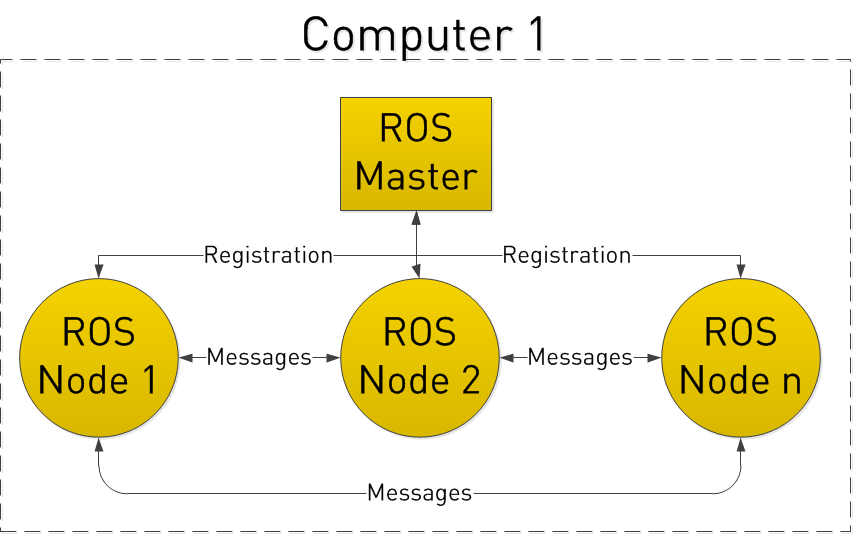
\includegraphics [width=0.5 \textwidth]{imgs/chapter2/rosgraph.png}}
\caption{ROS architecture overview \cite{rosbasics}}
\label{fig:rosgraph}
\end{figure}


